% !TEX program = xelatex
\documentclass[9pt, aspectratio=169]{beamer}
\usetheme{metropolis}
\usefonttheme{professionalfonts}

% --- Modern Font Setup ---
\usepackage[T1]{fontenc}
\usepackage{FiraSans}  % Modern, elegant sans-serif font family
\usepackage[scaled=0.95]{FiraMono}  % Matching monospace font

% Lighter, more refined font weights
\renewcommand{\seriesdefault}{l}  % Light weight as default
\renewcommand{\bfseries}{\fontseries{sb}\selectfont}  % Semi-bold instead of bold

% Custom font sizing - more refined
\setbeamerfont{title}{size=\Large, series=\fontseries{m}\selectfont}
\setbeamerfont{subtitle}{size=\normalsize, series=\fontseries{l}\selectfont}
\setbeamerfont{author}{size=\small, series=\fontseries{l}\selectfont}
\setbeamerfont{date}{size=\small, series=\fontseries{l}\selectfont}
\setbeamerfont{frametitle}{size=\normalsize, series=\fontseries{m}\selectfont}
\setbeamerfont{framesubtitle}{size=\footnotesize, series=\fontseries{l}\selectfont}
\setbeamerfont{block title}{size=\normalsize, series=\fontseries{m}\selectfont}
\setbeamerfont{block body}{size=\small}
\setbeamerfont{itemize/enumerate body}{size=\small}
\setbeamerfont{itemize/enumerate subbody}{size=\footnotesize}
\setbeamerfont{section in toc}{size=\normalsize, series=\fontseries{m}\selectfont}
\setbeamerfont{section title}{size=\Large, series=\fontseries{m}\selectfont}

% --- Color Definitions ---
% Primary Theme Colors
\definecolor{PrimaryColor}{RGB}{33,52,72}         % Deep navy
\definecolor{SecondaryColor}{RGB}{84,119,146}     % Desaturated blue-gray
\definecolor{AccentColor}{RGB}{100,156,165}       % Soft steel blue
\definecolor{black}{RGB}{0,0,0}
\definecolor{BackgroundColor}{RGB}{245,247,250}   % Very light cool gray/blue-tinted white
\definecolor{TextColor}{RGB}{40,55,70}            % Darker, cool-toned charcoal
\definecolor{LightGray}{RGB}{220,225,230}         % Soft, cool light gray
\definecolor{DarkGray}{RGB}{70,90,105}            % Cool-toned dark gray

% --- Theme Customization ---
\setbeamercolor{background canvas}{bg=BackgroundColor}
\setbeamercolor{normal text}{fg=TextColor}
\setbeamercolor{frametitle}{bg=PrimaryColor, fg=white}
\setbeamercolor{section in toc}{fg=PrimaryColor}
\setbeamercolor{block title}{bg=PrimaryColor!80, fg=white}
\setbeamercolor{block body}{bg=PrimaryColor!10}
\setbeamercolor{alerted text}{fg=AccentColor}
\setbeamercolor{itemize item}{fg=PrimaryColor}
\setbeamercolor{itemize subitem}{fg=SecondaryColor}

% Progress bar
\setbeamercolor{progress bar}{fg=AccentColor, bg=LightGray}

% --- Packages ---
\usepackage[utf8]{inputenc}
\usepackage{url}
\usepackage{booktabs}
\usepackage{amsmath, amssymb, amsfonts}
\usepackage{fontawesome5}
\usepackage{pifont}
\usepackage[most]{tcolorbox}
\tcbuselibrary{skins, listings}
\usepackage{colortbl}
\usepackage{array}
\usepackage{adjustbox}
\usepackage{ragged2e}

% --- Packages for plotting discrete and continuous signals and spectrums ---
\usepackage{tikz}
\usepackage{circuitikz} % Useful for signal processing block diagrams
\usepackage{pgfplots}
\usepackage{graphicx}
\usepackage{caption}
\usepackage{subcaption}

\usetikzlibrary{shapes.callouts, positioning, arrows.meta, shapes.geometric, shadows, calc, patterns, backgrounds, shadings, fit, chains, decorations.pathreplacing, intersections}
\usepgfplotslibrary{fillbetween}
\usepgfplotslibrary{polar}
\pgfplotsset{compat=1.18}
\pgfplotsset{
    plot coordinates/math parser=false,
    signal/.style={thick, color=PrimaryColor},
    spectrum/.style={thick, color=AccentColor},
    discrete/.style={ycomb, mark=*, mark options={fill=white, draw=PrimaryColor}, color=PrimaryColor, thick},
}

% --- Custom Commands ---
\newcommand{\cmark}{\textcolor{PrimaryColor}{\ding{51}}}
\newcommand{\xmark}{\textcolor{AccentColor}{\ding{55}}}
\newcommand{\highlight}[1]{\textcolor{PrimaryColor}{\textbf{#1}}}

% --- Custom tcolorbox environments ---
\newtcolorbox{conceptbox}[1]{
    colback=PrimaryColor!10,
    colframe=PrimaryColor,
    title=#1,
    fonttitle=\small\bfseries,
    fontupper=\small,
    rounded corners
}

\newtcolorbox{insightbox}[1]{
    colback=AccentColor!10,
    colframe=AccentColor,
    title=#1,
    fonttitle=\small\bfseries,
    fontupper=\small,
    rounded corners
}

\newtcolorbox{algorithmbox}[1]{
    colback=SecondaryColor!10,
    colframe=SecondaryColor,
    title=#1,
    fonttitle=\small\bfseries,
    fontupper=\small,
    rounded corners
}

\newtcblisting{codelistingbox}[2][]{
    colback=SecondaryColor!10,
    colframe=SecondaryColor,
    title=#2,
    fonttitle=\small\bfseries,
    rounded corners,
    listing only,
    listing options={
            language=#1,
            basicstyle=\ttfamily\footnotesize,
            keywordstyle=\color{PrimaryColor}\bfseries,
            commentstyle=\color{SecondaryColor}\itshape,
            stringstyle=\color{AccentColor},
            numbers=left,
            numberstyle=\tiny\color{DarkGray},
            stepnumber=1,
            showstringspaces=false,
            tabsize=4
        }
}


\subtitle{Signals and Linear Systems}
\date{}
\author{Ashrafur Rahman\\Lecturer, CSE, BUET}
\institute{ashrafur@cse.buet.ac.bd}


\title{The Laplace Transform}

\begin{document}

\pgfplotsset{every axis/.append style={tick style={draw=none}}}

\maketitle

\begin{frame}{Outline}
    \begin{itemize}
        \item \textbf{Introduction:} Generalizing the Fourier Transform
        \item \textbf{The Laplace Transform Definition}
        \item \textbf{The Region of Convergence (ROC):}
              \begin{itemize}
                  \item Left-Sided vs. Right-Sided Signals
                  \item Poles and Zeros
                  \item Properties of the ROC
              \end{itemize}
        \item \textbf{The Inverse Laplace Transform:}
              \begin{itemize}
                  \item Derivation \& Bromwich Contour Integration
                  \item Finding Inverse via Partial-Fraction Expansion
              \end{itemize}
    \end{itemize}
\end{frame}

\section{Introduction and Definition}

\begin{frame}{Introduction to the Laplace Transform}
    \begin{itemize}
        \item \textbf{Why general complex exponentials?}
              We learnt that a broad class of functions can be represented as a sum of complex exponentials $e^{j\omega t}$.
              Also, complex exponentials are eigenfunctions of LTI systems, i.e. $y(t) = H(j\omega)e^{j\omega t}$ for $x(t) = e^{j\omega t}$.
        \item Using the properties above, we expressed both input and output of an LTI system as a sum of complex exponentials.
        \item However, the eigenfunction property holds for \textit{any} arbitrary complex value $s = \sigma + j\omega$.
        \item This broader property leads to a generalization of the continuous-time Fourier transform known as the \textbf{Laplace Transform}.
        \item \textbf{Key Advantages of the Laplace Transform:}
              \begin{itemize}
                  \item It can analyze broad classes of signals and unstable systems where the Fourier transform \textit{does not exist}.
                  \item It provides deeper insights into the \textbf{stability or instability} of systems.
                  \item It maintains powerful algebraic properties, forming an essential set of tools for system analysis, especially \textbf{feedback systems}.
              \end{itemize}
    \end{itemize}
\end{frame}

\begin{frame}{System Response to Complex Exponentials}
    \begin{itemize}
        \item Recall that the response of a Linear Time-Invariant (LTI) system with impulse response $h(t)$ to a complex exponential input $x(t) = e^{st}$ is:
              \begin{align*}
                  y(t) & = x(t) * h(t) = \int_{-\infty}^{\infty} h(\tau) x(t-\tau) d\tau = \int_{-\infty}^{\infty} h(\tau) e^{s(t-\tau)} d\tau \\
                       & = e^{st} \int_{-\infty}^{\infty} h(\tau) e^{-s\tau} d\tau = H(s)e^{st}
              \end{align*}
        \item Here, the eigenvalue $H(s)$ corresponding to the eigenfunction $e^{st}$ is given by:
              \begin{equation*}
                  H(s) = \int_{-\infty}^{\infty} h(t) e^{-st} dt
              \end{equation*}
        \item For pure imaginary values $s = j\omega$, this integral is simply the \textbf{Fourier transform} of $h(t)$.
        \item For general complex values of $s$, this is referred to as the \textbf{Laplace transform} of the impulse response $h(t)$.
    \end{itemize}
\end{frame}

\begin{frame}{Definition of the Laplace Transform}
    \begin{itemize}
        \item Extending this beyond impulse responses, we define the Laplace transform of a general signal $x(t)$ as follows:
    \end{itemize}

    \vspace{0.2cm}
    \begin{conceptbox}{Laplace Transform}
        \vspace{-0.2cm}
        \begin{equation*}
            X(s) \triangleq \int_{-\infty}^{+\infty} x(t) e^{-st} dt
        \end{equation*}
    \end{conceptbox}

    \begin{itemize}
        \item The complex variable $s$ can be written in rectangular form as $s = \sigma + j\omega$, with $\sigma$ and $\omega$ representing the real and imaginary parts, respectively.
        \item We sometimes denote the Laplace transform in operator form as $X(s) = \mathcal{L}\{x(t)\}$ and the transform relationship as:
              \begin{equation*}
                  x(t) \stackrel{\mathcal{L}}{\overset{{\mathcal{L}}}{\longleftrightarrow}} X(s)
              \end{equation*}
    \end{itemize}
\end{frame}

\begin{frame}{Connection to the Fourier Transform}
    \begin{itemize}
        \item When the real part of $s$ is zero ($s = j\omega$), the Laplace transform becomes:
              \begin{equation*}
                  X(j\omega) = \int_{-\infty}^{+\infty} x(t) e^{-j\omega t} dt = \mathcal{F}\{x(t)\}
              \end{equation*}
        \item The Laplace transform bears a straightforward relationship to the Fourier transform for general $s = \sigma + j\omega$:
              \begin{align*}
                  X(\sigma + j\omega) & = \int_{-\infty}^{+\infty} x(t) e^{-(\sigma+j\omega)t} dt         \\
                                      & = \int_{-\infty}^{+\infty} [x(t) e^{-\sigma t}] e^{-j\omega t} dt
              \end{align*}
    \end{itemize}

    \vspace{0.2cm}
    \begin{insightbox}{Key Insight}
        The Laplace transform of $x(t)$ can be interpreted as the \textbf{Fourier transform of $x(t) e^{-\sigma t}$}.
        \vspace{0.2cm}

        The real exponential weighting $e^{-\sigma t}$ can force the signal into convergence, even if the Fourier transform of $x(t)$ alone does not converge!
    \end{insightbox}
\end{frame}

\section{Examples of the Laplace Transform}

\begin{frame}{Example 9.1: A Right-Sided Exponential Signal}
    \begin{columns}[T]
        \begin{column}{0.55\textwidth}
            \begin{itemize}
                \item Signal: $x(t) = e^{-at}u(t)$.
                \item Laplace transform:
                      \begin{align*}
                          X(s) & = \int_{0}^{\infty} e^{-(s+a)t} dt                       \\
                               & = \left[ -\frac{1}{s+a} e^{-(s+a)t} \right]_{0}^{\infty}
                      \end{align*}
                \item We evaluate the upper limit:
                      \begin{align*}
                          \lim_{t \to \infty} e^{-(s+a)t} = \lim_{t \to \infty} e^{-(\sigma+a)t} e^{-j\omega t} = 0 \text{ if } \sigma+a > 0
                      \end{align*}
                \item Hence the integral converges if $\text{Re}\{s\} > -a$.
                \item Evaluating the lower limit at $t=0$ yields:
                      \begin{equation*}
                          X(s) = \frac{1}{s+a}, \quad \text{Re}\{s\} > -a
                      \end{equation*}
            \end{itemize}
        \end{column}
        \begin{column}{0.45\textwidth}
            \vspace{-0.3cm}
            \textbf{Time Domain $x(t)$}\\
            \begin{center}
                \begin{tikzpicture}
                    \begin{axis}[tick style={draw=none},
                        width=0.9\textwidth, height=3.2cm,
                        axis lines=middle, axis line style={-{Latex[length=2mm]}},
                        xmin=-2, xmax=4, ymin=-0.2, ymax=1.2,
                        xtick=\empty, ytick={1}, yticklabels={$1$},
                        xlabel={$t$}, ylabel={$x(t)$},
                        xlabel style={anchor=west, at={(axis cs:4.2,0)}},
                        ylabel style={anchor=south, at={(axis cs:0,1.3)}},
                        declare function={sig(\t) = \t >= 0 ? exp(-0.8*\t) : 0;}
                        ]
                        \addplot[thick, PrimaryColor, domain=-2:4, samples=150] {sig(x)};
                        \draw[dashed, PrimaryColor, thick] (axis cs:0,0) -- (axis cs:0,1);
                    \end{axis}
                \end{tikzpicture}
            \end{center}
            \textbf{Laplace Domain ($s$-plane)}\\
            \begin{center}
                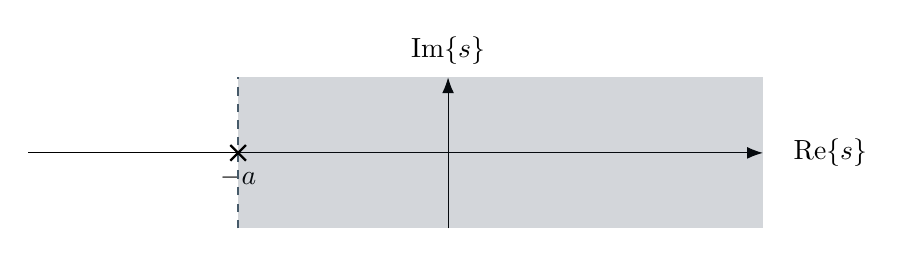
\begin{tikzpicture}
                    \begin{axis}[tick style={draw=none},
                        width=0.9\textwidth, height=3.5cm,
                        axis lines=middle, axis line style={-{Latex[length=2mm]}},
                        xmin=-4, xmax=3, ymin=-2.5, ymax=2.5,
                        xtick={-2}, xticklabels={$-a$},
                        ytick=\empty,
                        xlabel={$\text{Re}\{s\}$}, ylabel={$\text{Im}\{s\}$},
                        xlabel style={anchor=west, at={(axis cs:3.2,0)}},
                        ylabel style={anchor=south, at={(axis cs:0,2.6)}},
                        clip=false
                        ]
                        \fill[PrimaryColor, fill opacity=0.2] (axis cs:-2,-2.5) rectangle (axis cs:3,2.5);
                        \draw[dashed, thick, DarkGray] (axis cs:-2,-2.5) -- (axis cs:-2,2.5);
                        \addplot[only marks, mark=x, mark options={scale=2, thick}] coordinates {(-2,0)};
                    \end{axis}
                \end{tikzpicture}
            \end{center}
        \end{column}
    \end{columns}
\end{frame}

\begin{frame}{Example 9.2: A Left-Sided Exponential Signal}
    \begin{columns}[T]
        \begin{column}{0.55\textwidth}
            \begin{itemize}
                \item Signal: $x(t) = -e^{-at}u(-t)$.
                \item Laplace transform:
                      \begin{align*}
                          X(s) & = \int_{-\infty}^{0} -e^{-(s+a)t} dt                     \\
                               & = \left[ \frac{1}{s+a} e^{-(s+a)t} \right]_{-\infty}^{0}
                      \end{align*}
                \item For convergence at $t \to -\infty$, exponentials must decay:
                      \begin{equation*}
                          \sigma + a < 0 \implies \text{Re}\{s\} < -a
                      \end{equation*}
                \item Evaluating yields the \textit{exact same} algebraic expression:
                      \begin{equation*}
                          X(s) = \frac{1}{s+a}, \quad \text{Re}\{s\} < -a
                      \end{equation*}
            \end{itemize}
        \end{column}
        \begin{column}{0.45\textwidth}
            \vspace{-0.3cm}
            \textbf{Time Domain $x(t)$}\\
            \begin{center}
                \begin{tikzpicture}
                    \begin{axis}[tick style={draw=none},
                        width=0.9\textwidth, height=3.2cm,
                        axis lines=middle, axis line style={-{Latex[length=2mm]}},
                        xmin=-4, xmax=2, ymin=-3.5, ymax=0.5,
                        xtick=\empty, ytick={-1}, yticklabels={$-1$},
                        xlabel={$t$}, ylabel={$x(t)$},
                        xlabel style={anchor=west, at={(axis cs:2.2,0)}},
                        ylabel style={anchor=south, at={(axis cs:0,0.3)}},
                        declare function={sig(\t) = \t <= 0 ? -exp(-0.8*\t) : 0;}
                        ]
                        \addplot[thick, SecondaryColor, domain=-4:2, samples=150] {sig(x)};
                        \draw[dashed, SecondaryColor, thick] (axis cs:0,0) -- (axis cs:0,-1);
                    \end{axis}
                \end{tikzpicture}
            \end{center}
            \textbf{Laplace Domain ($s$-plane)}\\
            \begin{center}
                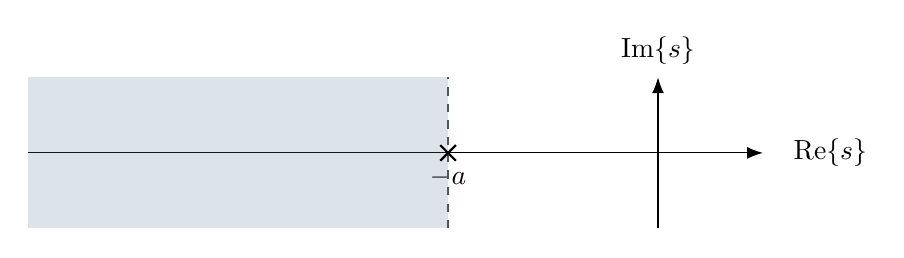
\begin{tikzpicture}
                    \begin{axis}[tick style={draw=none},
                        width=0.9\textwidth, height=3.5cm,
                        axis lines=middle, axis line style={-{Latex[length=2mm]}},
                        xmin=-6, xmax=1, ymin=-2.5, ymax=2.5,
                        xtick={-2}, xticklabels={$-a$},
                        ytick=\empty,
                        xlabel={$\text{Re}\{s\}$}, ylabel={$\text{Im}\{s\}$},
                        xlabel style={anchor=west, at={(axis cs:1.2,0)}},
                        ylabel style={anchor=south, at={(axis cs:0,2.6)}},
                        clip=false
                        ]
                        \fill[SecondaryColor, fill opacity=0.2] (axis cs:-6,-2.5) rectangle (axis cs:-2,2.5);
                        \draw[dashed, thick, DarkGray] (axis cs:-2,-2.5) -- (axis cs:-2,2.5);
                        \addplot[only marks, mark=x, mark options={scale=2, thick}] coordinates {(-2,0)};
                    \end{axis}
                \end{tikzpicture}
            \end{center}
        \end{column}
    \end{columns}
\end{frame}


\begin{frame}{The $s$-plane and Region of Convergence (ROC)}
    \begin{columns}[T]
        \begin{column}{0.55\textwidth}
            \begin{itemize}
                \item The Laplace transform depends on the complex variable $s = \sigma + j\omega$.
                \item We visualize this using a 2D plot called the \textbf{$s$-plane}:
                      \begin{itemize}
                          \item \textbf{Horizontal axis ($\sigma$):} Real part of $s$.
                          \item \textbf{Vertical axis ($j\omega$):} Imaginary part of $s$.
                      \end{itemize}
                \item \textbf{Region of Convergence (ROC):} The specific set of values in the $s$-plane for which the integral $X(s)$ converges to a finite value.
                      \begin{itemize}
                          \item Unlike Fourier Transform, the ROC is an important part of the Laplace Transform.
                          \item As we saw in the previous two example, even though the algebraic expression for $X(s)$ was the same, the ROC was different.
                      \end{itemize}
                \item \textbf{Relation to Fourier:} The $j\omega$-axis (where $\sigma=0$) corresponds to the Fourier transform. If the ROC includes this vertical axis, the Fourier transform of the signal converges!
            \end{itemize}
        \end{column}
        \begin{column}{0.45\textwidth}
            \vspace{-0.3cm}
            \begin{center}
                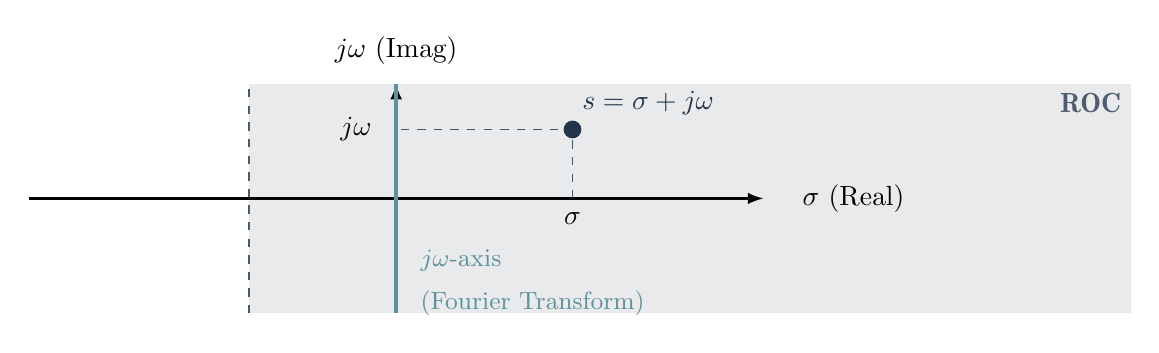
\begin{tikzpicture}
                    \begin{axis}[tick style={draw=none},
                        width=0.9\textwidth, height=4.5cm,
                        axis lines=middle, axis line style={-{Latex[length=2mm]}, thick},
                        xmin=-2.5, xmax=2.5, ymin=-2.5, ymax=2.5,
                        xtick=\empty, ytick=\empty,
                        xlabel={$\sigma$ (Real)}, ylabel={$j\omega$ (Imag)},
                        xlabel style={anchor=west, at={(axis cs:2.7,0)}},
                        ylabel style={anchor=south, at={(axis cs:0,2.7)}},
                        clip=false
                        ]

                        % Emphasize the jw axis first
                        \draw[ultra thick, AccentColor] (axis cs:0,-2.5) -- (axis cs:0,2.5);
                        \node[AccentColor, anchor=south west] at (axis cs:0.1, -1.8) {\small $j\omega$-axis};
                        \node[AccentColor, anchor=north west] at (axis cs:0.1, -1.8) {\small (Fourier Transform)};

                        % Generic point
                        \addplot[only marks, mark=*, mark options={scale=1.5, PrimaryColor}] coordinates {(1.2, 1.5)};
                        \draw[dashed, DarkGray] (axis cs:1.2,0) -- (axis cs:1.2,1.5) -- (axis cs:0,1.5);
                        \node[PrimaryColor, anchor=south west] at (axis cs:1.2, 1.6) {$s = \sigma + j\omega$};
                        \node[anchor=north] at (axis cs:1.2, -0.1) {$\sigma$};
                        \node[anchor=east] at (axis cs:-0.1, 1.5) {$j\omega$};


                        \fill[PrimaryColor, fill opacity=0.1] (axis cs:-1,-2.5) rectangle (axis cs:5,2.5);
                        \draw[dashed, thick, DarkGray] (axis cs:-1,-2.5) -- (axis cs:-1,2.5);
                        \node[PrimaryColor!80, anchor=north east] at (axis cs:5, 2.5) {\textbf{ROC}};

                    \end{axis}
                \end{tikzpicture}
            \end{center}
        \end{column}
    \end{columns}
\end{frame}


\begin{frame}{Rational Laplace Transforms}
    \begin{itemize}
        \item Many important LTI systems and signals have Laplace transforms that are \textbf{rational functions} of $s$, meaning they are ratios of two polynomials in $s$.
        \item For a signal $x(t)$ with a rational Laplace transform, we can express $X(s)$ as:
              \begin{equation*}
                  X(s) = \frac{N(s)}{D(s)}
              \end{equation*}
        \item \textbf{Zeros} are the values of $s$ for which $N(s) = 0$ (so $X(s) = 0$). We denote roots of the numerator with an \textbf{o} ($\circ$) on the $s$-plane.
        \item \textbf{Poles} are the values of $s$ for which $D(s) = 0$ (so $X(s) \to \infty$). We denote roots of the denominator with an \textbf{x} ($\times$).
    \end{itemize}
\end{frame}

\begin{frame}{Example 9.3: Sum of Two Exponentials}
    \begin{columns}[T]
        \begin{column}{0.5\textwidth}
            \begin{itemize}
                \item Signal: $x(t) = 3e^{-2t}u(t) - 2e^{-t}u(t)$
                \item Using linearity and Example 9.1:
                      \begin{align*}
                          3e^{-2t}u(t) & \overset{{\mathcal{L}}}{\longleftrightarrow} \frac{3}{s+2}, \quad \text{Re}\{s\} > -2  \\
                          -2e^{-t}u(t) & \overset{{\mathcal{L}}}{\longleftrightarrow} \frac{-2}{s+1}, \quad \text{Re}\{s\} > -1
                      \end{align*}
                \item Combined transform:
                      \begin{equation*}
                          X(s) = \frac{3}{s+2} - \frac{2}{s+1} = \frac{s - 1}{(s+1)(s+2)}
                      \end{equation*}
                \item \textbf{ROC:} Intersection yields $\text{Re}\{s\} > -1$.
                \item \textbf{Zeros:} $s = 1$, \quad \textbf{Poles:} $s = -1, -2$
            \end{itemize}
        \end{column}
        \begin{column}{0.5\textwidth}
            \begin{center}
                \vspace{0.6cm}
                \textbf{Pole-Zero Plot ($s$-plane)}
                \vspace{0.1cm}

                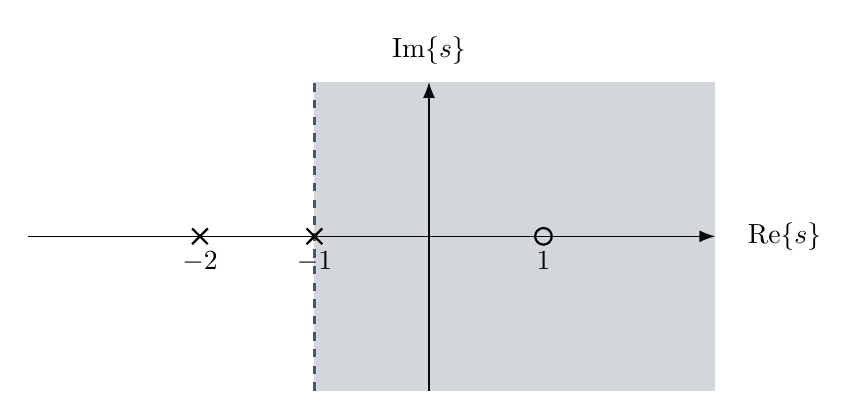
\begin{tikzpicture}
                    \begin{axis}[tick style={draw=none},
                        width=0.85\textwidth, height=5.5cm,
                        axis lines=middle, axis line style={-{Latex[length=2mm]}},
                        xmin=-3.5, xmax=2.5, ymin=-2, ymax=2,
                        xtick={-2, -1, 1},
                        ytick=\empty,
                        xlabel={$\text{Re}\{s\}$}, ylabel={$\text{Im}\{s\}$},
                        xlabel style={anchor=west, at={(axis cs:2.7,0)}},
                        ylabel style={anchor=south, at={(axis cs:0,2.1)}},
                        clip=false
                        ]
                        \fill[PrimaryColor, fill opacity=0.2] (axis cs:-1,-2) rectangle (axis cs:2.5,2);
                        \draw[dashed, thick, DarkGray] (axis cs:-1,-2) -- (axis cs:-1,2);
                        \addplot[only marks, mark=x, mark options={scale=2, thick}] coordinates {(-1,0) (-2,0)};
                        \addplot[only marks, mark=o, mark options={scale=1.5, thick}] coordinates {(1,0)};
                    \end{axis}
                \end{tikzpicture}
            \end{center}
            \vspace{-0.2cm}
            \small\textit{Note: ROC bounded by the right pole ($s=-1$).}
        \end{column}
    \end{columns}
\end{frame}

\begin{frame}{Example 9.4: Decay with Oscillation}
    \begin{columns}[T]
        \begin{column}{0.55\textwidth}
            \begin{itemize}
                \item Signal: $x(t) = e^{-2t}u(t) + e^{-t}(\cos 3t)u(t)$.
                \item Expanding $\cos$ via Euler's relation:
                      \begin{equation*}
                          x(t) = e^{-2t}u(t) + \frac{1}{2}e^{-(1-3j)t}u(t) + \frac{1}{2}e^{-(1+3j)t}u(t)
                      \end{equation*}
                \item Laplace transforms of individual terms:
                      \begin{align*}
                          X_1(s) & = \frac{1}{s+2}, \quad        &  & \text{Re}\{s\} > -2 \\
                          X_2(s) & = \frac{1/2}{s+(1-3j)}, \quad &  & \text{Re}\{s\} > -1 \\
                          X_3(s) & = \frac{1/2}{s+(1+3j)}, \quad &  & \text{Re}\{s\} > -1
                      \end{align*}
                \item Combining algebraically gives:
                      \begin{equation*}
                          X(s) = \frac{2s^2 + 5s + 12}{(s+2)(s^2 + 2s + 10)}, \quad \text{Re}\{s\} > -1
                      \end{equation*}
                \item \textbf{Poles:} $s = -2, s = -1 \pm 3j$. \textbf{Zeros:} $s \approx -1.25 \pm 2.11j$
            \end{itemize}
        \end{column}
        \begin{column}{0.45\textwidth}
            \begin{center}
                \vspace{0.6cm}
                \textbf{Pole-Zero Plot ($s$-plane)}
                \vspace{0.1cm}

                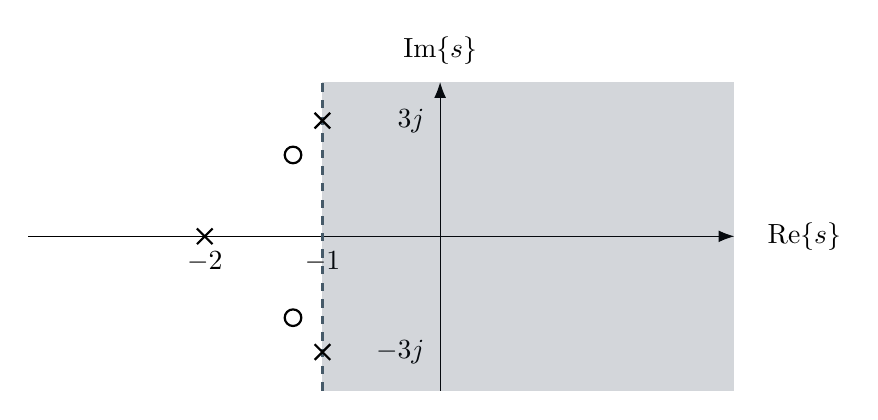
\begin{tikzpicture}
                    \begin{axis}[tick style={draw=none},
                        width=0.87\textwidth, height=5.5cm,
                        axis lines=middle, axis line style={-{Latex[length=2mm]}},
                        xmin=-3.5, xmax=2.5, ymin=-4, ymax=4,
                        xtick={-2, -1},
                        ytick={-3, 3}, yticklabels={$-3j$, $3j$},
                        xlabel={$\text{Re}\{s\}$}, ylabel={$\text{Im}\{s\}$},
                        xlabel style={anchor=west, at={(axis cs:2.7,0)}},
                        ylabel style={anchor=south, at={(axis cs:0,4.2)}},
                        clip=false
                        ]
                        \fill[PrimaryColor, fill opacity=0.2] (axis cs:-1,-4) rectangle (axis cs:2.5,4);
                        \draw[dashed, thick, DarkGray] (axis cs:-1,-4) -- (axis cs:-1,4);

                        % Poles
                        \addplot[only marks, mark=x, mark options={scale=2, thick}] coordinates {(-2,0) (-1,3) (-1,-3)};
                        % Zeros
                        \addplot[only marks, mark=o, mark options={scale=1.5, thick}] coordinates {(-1.25, 2.11) (-1.25, -2.11)};
                    \end{axis}
                \end{tikzpicture}
            \end{center}
        \end{column}
    \end{columns}
\end{frame}

\begin{frame}{Example 9.5: A Signal with an Impulse}
    \begin{columns}[T]
        \begin{column}{0.55\textwidth}
            \begin{itemize}
                \item Signal: $x(t) = \delta(t) - \frac{4}{3}e^{-t}u(t) + \frac{1}{3}e^{2t}u(t)$
                \item The Laplace transform of the unit impulse converges for the \textit{entire} $s$-plane:
                      \begin{equation*}
                          \mathcal{L}\{\delta(t)\} = \int_{-\infty}^{\infty} \delta(t)e^{-st} dt = 1
                      \end{equation*}
                \item Thus, the total transform is:
                      \begin{equation*}
                          X(s) = 1 - \frac{4/3}{s+1} + \frac{1/3}{s-2}
                      \end{equation*}
                \item Expanding and keeping common denominator:
                      \begin{equation*}
                          X(s) = \frac{3s^2-6s+3}{3(s+1)(s-2)} = \frac{(s-1)^2}{(s+1)(s-2)}
                      \end{equation*}
                \item \textbf{ROC:} Intersection of conditions ($\text{Re}\{s\}>-\infty$, $\text{Re}\{s\}>-1$, $\text{Re}\{s\}>2$) yields $\text{Re}\{s\} > 2$.
            \end{itemize}
        \end{column}
        \begin{column}{0.45\textwidth}
            \begin{center}
                \vspace{0.6cm}
                \textbf{Pole-Zero Plot ($s$-plane)}
                \vspace{0.1cm}

                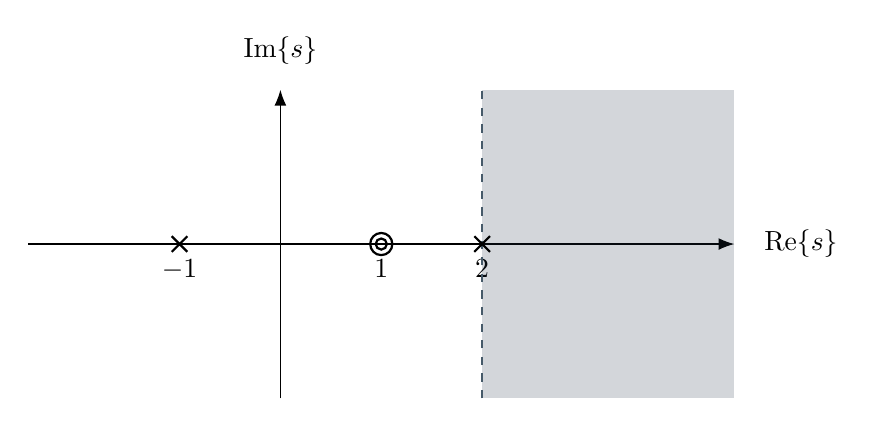
\begin{tikzpicture}
                    \begin{axis}[tick style={draw=none},
                        width=0.87\textwidth, height=5.5cm,
                        axis lines=middle, axis line style={-{Latex[length=2mm]}},
                        xmin=-2.5, xmax=4.5, ymin=-2, ymax=2,
                        xtick={-1, 1, 2},
                        ytick=\empty,
                        xlabel={$\text{Re}\{s\}$}, ylabel={$\text{Im}\{s\}$},
                        xlabel style={anchor=west, at={(axis cs:4.7,0)}},
                        ylabel style={anchor=south, at={(axis cs:0,2.2)}},
                        clip=false
                        ]
                        \fill[PrimaryColor, fill opacity=0.2] (axis cs:2,-2) rectangle (axis cs:4.5,2);
                        \draw[dashed, thick, DarkGray] (axis cs:2,-2) -- (axis cs:2,2);

                        % Poles
                        \addplot[only marks, mark=x, mark options={scale=2, thick}] coordinates {(-1,0) (2,0)};
                        % Double Zero
                        \addplot[only marks, mark=o, mark options={scale=2, thick}] coordinates {(1,0)};
                        \addplot[only marks, mark=o, mark options={scale=1, thick}] coordinates {(1,0)};
                    \end{axis}
                \end{tikzpicture}
            \end{center}
        \end{column}
    \end{columns}
\end{frame}

\section{Properties of the Region of Convergence (ROC)}

\begin{frame}{ROC Property 1 and 2}
    \begin{tcolorbox}[colframe=PrimaryColor, colback=PrimaryColor!10]
        \textbf{Property 1:} The ROC of $X(s)$ consists of strips parallel to the $j\omega$-axis in the $s$-plane.
    \end{tcolorbox}
    \vspace{0.2cm}
    \textit{Justification:} The Laplace transform converges if $x(t)e^{-st}$ is absolutely integrable. If $\sigma + j\omega$ is in the ROC, then
    \begin{align*}
        \int_{-\infty}^{\infty} \left|x(t)e^{-(\sigma + j\omega)t}\right| dt
        = \int_{-\infty}^{\infty} \left|x(t)\right|e^{-\sigma t}  dt < \infty \qquad \text {since } \left|e^{-j\omega t}\right| = 1
    \end{align*}
    Thus, convergence depends entirely on $\sigma = \text{Re}\{s\}$. If a point $\sigma + j\omega$ converges, all points on the vertical line $\sigma$ must also converge.
    \vspace{0.4cm}

    \begin{tcolorbox}[colframe=PrimaryColor, colback=PrimaryColor!10]
        \textbf{Property 2:} For rational Laplace transforms, the ROC does not contain any poles.
    \end{tcolorbox}
    \vspace{0.2cm}
    \textit{Justification:} By definition, $X(s)$ evaluates to infinity at a pole. Since convergence requires $X(s)$ to be finite, the integral naturally diverges at the exact location of any pole.
\end{frame}

\begin{frame}{ROC Property 3: Finite-Duration Signals}
    \begin{tcolorbox}[colframe=PrimaryColor, colback=PrimaryColor!10]
        \textbf{Property 3:} If $x(t)$ is of finite duration and is absolutely integrable, then the ROC is the entire $s$-plane.
    \end{tcolorbox}
    \vspace{0.2cm}
    \textit{Justification:} Let $x(t) \neq 0$ only in $T_1 < t < T_2$. The absolute integrability integral becomes:
    \begin{equation*}
        \int_{T_1}^{T_2} |x(t)| e^{-\sigma t} dt
    \end{equation*}
    Since the interval is finite, the maximum value of $e^{-\sigma t}$ over $[T_1, T_2]$ is bounded for any finite $\sigma$:
    \begin{align*}
        \int_{T_1}^{T_2} |x(t)| e^{-\sigma t} dt \le e^{-\sigma T_{max}} \int_{T_1}^{T_2} |x(t)| dt < \infty
        \qquad \text{where } T_{max} = \begin{cases}
                                           T_1 & \text{if } \sigma > 0 \\
                                           T_2 & \text{if } \sigma < 0
                                       \end{cases}
    \end{align*}
    This is because if $\sigma > 0$, $e^{-\sigma t}$ decays, so $e^{-\sigma T_1}$ is the largest value of $e^{-\sigma t}$ over $[T_1, T_2]$.
    If $\sigma < 0$, $e^{-\sigma t}$ grows, so $e^{-\sigma T_2}$ is the largest value of $e^{-\sigma t}$ over $[T_1, T_2]$.

    Thus, convergence spans from $-\infty < \sigma < \infty$.
\end{frame}

\begin{frame}{Example 9.6: An Apparent Pole Cancellation}
    \begin{columns}[T]
        \begin{column}{0.55\textwidth}
            \begin{itemize}
                \item Consider a finite-duration signal:
                      \begin{equation*}
                          x(t) = \begin{cases} e^{-at}, & 0 < t < T \\ 0, & \text{otherwise} \end{cases}
                      \end{equation*}
                \item Evaluating the transform:
                      \begin{align*}
                          X(s) & = \int_{0}^{T} e^{-at} e^{-st} dt             \\
                               & = \frac{1}{s+a}\left[ 1 - e^{-(s+a)T} \right]
                      \end{align*}
                \item By \textbf{Property 3}, the ROC is the \textit{entire} $s$-plane.
                \item \textbf{But wait:} There appears to be a pole at $s = -a$. Isn't that a contradiction?
                \item No! At $s = -a$, both numerator and denominator evaluate to $0$. Using L'Hôpital's rule:
                      \begin{align*}
                          \lim_{s \to -a} X(s) & = \lim_{s \to -a} \left[ \frac{\frac{d}{ds}\left(1 - e^{-(s+a)T}\right)}{\frac{d}{ds}(s+a)} \right] \\
                                               & = \lim_{s \to -a} T e^{-aT}e^{-sT} = T
                      \end{align*}
                \item Thus, $X(-a) = T$, meaning the "pole" is perfectly canceled by a zero at $s = -a$.
            \end{itemize}
        \end{column}
        \begin{column}{0.45\textwidth}
            \begin{center}
                \vspace{-0.3cm}
                \textbf{Time Domain $x(t)$}\\
                \vspace{0.1cm}

                \begin{tikzpicture}
                    \begin{axis}[tick style={draw=none},
                        width=0.9\textwidth, height=4.5cm,
                        axis lines=middle, axis line style={-{Latex[length=2mm]}},
                        xmin=-1, xmax=5, ymin=-0.2, ymax=1.2,
                        xtick={0, 3}, xticklabels={$0$, $T$},
                        ytick={1}, yticklabels={$1$},
                        xlabel={$t$}, ylabel={$x(t)$},
                        xlabel style={anchor=west, at={(axis cs:5.3,0)}},
                        ylabel style={anchor=south, at={(axis cs:0,1.3)}},
                        clip=false
                        ]

                        % Draw zero lines before and after
                        \draw[thick, PrimaryColor] (axis cs:-1,0) -- (axis cs:0,0);
                        \draw[thick, PrimaryColor] (axis cs:3,0) -- (axis cs:5,0);

                        % Draw the exponential pulse
                        \addplot[thick, PrimaryColor, domain=0:3, samples=100] {exp(-0.6*x)};

                        % Vertical drop at T
                        \draw[thick, PrimaryColor, dashed] (axis cs:3,0.165) -- (axis cs:3,0);

                        % Marker at origin
                        \addplot[only marks, mark=*, mark options={scale=1.2}, PrimaryColor] coordinates {(0,1)};
                        \addplot[only marks, mark=o, mark options={scale=1.5, thick}, PrimaryColor] coordinates {(3,0.165)};
                    \end{axis}
                \end{tikzpicture}
                \vspace{0.6cm}\\
                \textit{\small A finite-duration signal cannot have any true poles because the integrals remain strictly bounded over the finite interval.}
            \end{center}
        \end{column}
    \end{columns}
\end{frame}

\begin{frame}[fragile]{ROC Property 4: Right-Sided Signals}
    \begin{tcolorbox}[colframe=PrimaryColor, colback=PrimaryColor!10]
        \textbf{Property 4:} If $x(t)$ is \textit{right-sided}, and if the line $\text{Re}\{s\} = \sigma_0$ is in the ROC, then all values of $s$ for which $\text{Re}\{s\} > \sigma_0$ will also be in the ROC.
    \end{tcolorbox}
    \vspace{0.2cm}
    \textit{Justification:} A right-sided signal is zero prior to some finite time $T_1$.

    If $x(t)e^{-\sigma_0 t}$ converges, then $x(t)e^{-\sigma t}$ will decrease even faster as $t \to +\infty$ whenever $\sigma_1 > \sigma_0$, as shown in the figure. More formally,
    \begin{align*}
        \int_{T_1}^\infty |x(t)|e^{-\sigma_1 t} dt = \int_{T_1}^\infty |x(t)|e^{-\sigma_0 t} e^{-(\sigma_1 - \sigma_0)t} dt
        \le e^{-(\sigma_1 - \sigma_0)T_1} \int_{T_1}^\infty |x(t)|e^{-\sigma_0 t} dt < \infty
    \end{align*}
    As $e^{-(\sigma_1 - \sigma_0)T_1} $ and $\int_{T_1}^\infty |x(t)|e^{-\sigma_0 t} dt$ are finite.
    \begin{columns}
        \begin{column}{0.5\textwidth}
            \begin{center}
                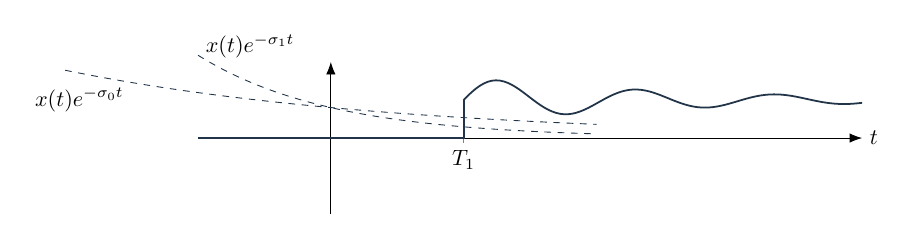
\begin{tikzpicture}[scale=0.8]
                    \begin{axis}[
                        width=\textwidth, height=4cm,
                        axis lines=middle, axis line style={-{Latex[length=2mm]}},
                        xmin=-1, xmax=4, ymin=-1, ymax=1,
                        xtick={1}, xticklabels={$T_1$},
                        ytick=\empty,
                        xlabel={$t$}, clip=false,
                        xlabel style={anchor=west}
                        ]
                        \addplot[thick, PrimaryColor, domain=1:4, samples=100] {0.5+0.3*exp(-0.6*(x-1))*sin(deg(6*(x-1)))};

                        \addplot[dashed, PrimaryColor, domain=-2:2, samples=100] {0.4*exp(-0.4*x)};
                        \addplot[dashed, PrimaryColor, domain=-1:2, samples=100] {0.4*exp(-x)};
                        \node[left] at (axis cs:-1.5,0.5) {$x(t)e^{-\sigma_0 t}$};
                        \node[right] at (axis cs:-1,1.2) {$x(t)e^{-\sigma_1 t}$};

                        \draw[thick, PrimaryColor] (axis cs:-1,0) -- (axis cs:1,0) -- (axis cs:1,0.5);
                    \end{axis}
                \end{tikzpicture}
            \end{center}
        \end{column}
        \begin{column}{0.5\textwidth}
            \begin{center}
                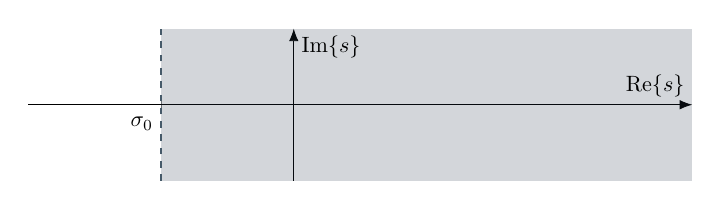
\begin{tikzpicture}[scale=0.8]
                    \begin{axis}[
                        width=\textwidth, height=4cm,
                        axis lines=middle, axis line style={-{Latex[length=2mm]}},
                        xmin=-2, xmax=3, ymin=-2, ymax=2,
                        xtick={-1}, xticklabels={$\sigma_0$},
                        xticklabel style={anchor=north east},
                        ytick=\empty,
                        xlabel={$\text{Re}\{s\}$}, ylabel={$\text{Im}\{s\}$}, clip=false
                        ]
                        \fill[PrimaryColor, fill opacity=0.2] (axis cs:-1,-2) rectangle (axis cs:3,2);
                        \draw[dashed, thick, DarkGray] (axis cs:-1,-2) -- (axis cs:-1,2);
                    \end{axis}
                \end{tikzpicture}
            \end{center}
        \end{column}
    \end{columns}
\end{frame}

\begin{frame}[fragile]{ROC Property 5: Left-Sided Signals}
    \begin{tcolorbox}[colframe=PrimaryColor, colback=PrimaryColor!10]
        \textbf{Property 5:} If $x(t)$ is \textit{left-sided}, and if the line $\text{Re}\{s\} = \sigma_0$ is in the ROC, then all values of $s$ for which $\text{Re}\{s\} < \sigma_0$ will also be in the ROC.
    \end{tcolorbox}
    \vspace{0.2cm}
    \textit{Justification:} Analogous to Property 4, the signal extends to $t \to -\infty$.
    For convergence, we need exponential compounding to die out in the negative time direction, which occurs when $\sigma_1 < \sigma_0$.
    \begin{columns}
        \begin{column}{0.5\textwidth}
            \begin{center}
                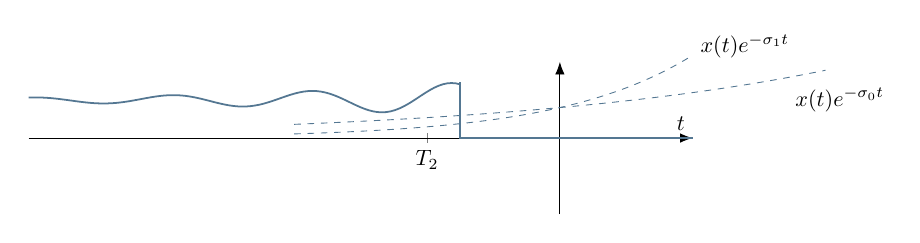
\begin{tikzpicture}[scale=0.8]
                    \begin{axis}[
                        width=\textwidth, height=4cm,
                        axis lines=middle, axis line style={-{Latex[length=2mm]}},
                        xmin=-4, xmax=1, ymin=-1, ymax=1,
                        xtick={-1}, xticklabels={$T_2$},
                        ytick=\empty,
                        xlabel={$t$}, clip=false
                        ]
                        \addplot[thick, SecondaryColor, domain=-4:-0.75, samples=100] {0.5+0.2*exp(0.6*(x+1))*sin(deg(6*(x-1)))};
                        \addplot[dashed, SecondaryColor, domain=-2:2, samples=100] {0.4*exp(0.4*x)};
                        \addplot[dashed, SecondaryColor, domain=-2:1, samples=100] {0.4*exp(x)};
                        \node[left] at (axis cs:2.5,0.5) {$x(t)e^{-\sigma_0 t}$};
                        \node[right] at (axis cs:1,1.2) {$x(t)e^{-\sigma_1 t}$};
                        \draw[thick, SecondaryColor] (axis cs:-0.75,0.73) -- (axis cs:-0.75,0) -- (axis cs:1,0);
                    \end{axis}
                \end{tikzpicture}
            \end{center}
        \end{column}
        \begin{column}{0.5\textwidth}
            \begin{center}
                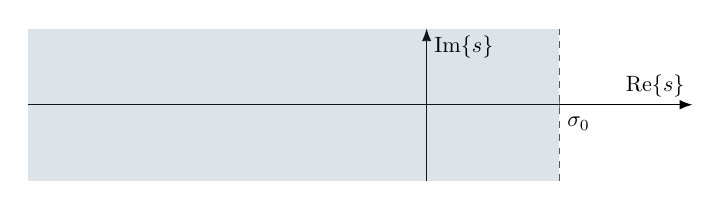
\begin{tikzpicture}[scale=0.8]
                    \begin{axis}[
                        width=\textwidth, height=4cm,
                        axis lines=middle, axis line style={-{Latex[length=2mm]}},
                        xmin=-3, xmax=2, ymin=-2, ymax=2,
                        xtick={1}, xticklabels={$\sigma_0$},
                        xticklabel style={anchor=north west},
                        ytick=\empty,
                        xlabel={$\text{Re}\{s\}$}, ylabel={$\text{Im}\{s\}$}, clip=false
                        ]
                        \fill[SecondaryColor, fill opacity=0.2] (axis cs:-3,-2) rectangle (axis cs:1,2);
                        \draw[dashed, thick, DarkGray] (axis cs:1,-2) -- (axis cs:1,2);
                    \end{axis}
                \end{tikzpicture}
            \end{center}
        \end{column}
    \end{columns}
\end{frame}

\begin{frame}[fragile]{ROC Property 6: Two-Sided Signals}
    \begin{tcolorbox}[colframe=PrimaryColor, colback=PrimaryColor!10]
        \textbf{Property 6:} If $x(t)$ is two-sided, and if the line $\text{Re}\{s\} = \sigma_0$ is in the ROC, then the ROC will consist of a \textit{strip} in the $s$-plane that includes the line $\text{Re}\{s\} = \sigma_0$.
    \end{tcolorbox}
    \begin{columns}
        \begin{column}{0.5\textwidth}
            \begin{center}
                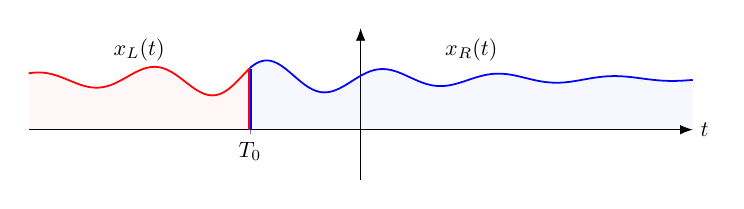
\begin{tikzpicture}[scale=0.8]
                    \begin{axis}[
                        width=\textwidth, height=4cm,
                        axis lines=middle, axis line style={-{Latex[length=2mm]}},
                        xmin=-3, xmax=3, ymin=-0.5, ymax=1,
                        xtick=\empty, ytick=\empty,
                        xlabel={$t$}, clip=false,
                        xtick={-1}, xticklabels={$T_0$},
                        xlabel style={anchor=west}
                        ]
                        \addplot[thick, red, domain=-3:-1, samples=150] {0.5+0.2*exp(-0.6*abs(x+1))*sin(deg(6*(x-1)))};
                        \addplot[thick, blue, domain=-1:3, samples=150] {0.5+0.2*exp(-0.6*abs(x+1))*sin(deg(6*(x-1)))};
                        \addplot[
                            opacity=0,
                            domain=-3:-1,
                            samples=150,
                            fill=red!60,
                            fill opacity=0.05
                        ] {0.5+0.2*exp(-0.6*abs(x+1))*sin(deg(6*(x-1)))}
                        \closedcycle;
                        \addplot[
                            opacity=0,
                            domain=-1:3,
                            samples=150,
                            fill=blue!60,
                            fill opacity=0.05
                        ] {0.5+0.2*exp(-0.6*abs(x+1))*sin(deg(6*(x-1)))}
                        \closedcycle;
                        \draw[thick, red] (axis cs:-1.01,0) -- (axis cs:-1.01,0.6);
                        \draw[thick, blue] (axis cs:-0.99,0) -- (axis cs:-0.99,0.6);
                        \node[above] at (axis cs:1,0.6) {$x_R(t)$};
                        \node[above] at (axis cs:-2,0.6) {$x_L(t)$};


                    \end{axis}
                \end{tikzpicture}
            \end{center}
            \vspace{-0.2cm}

            \footnotesize
            \begin{itemize}
                \item $x(t)$ can be divided at any arbitrary $T_0$ into $x_L(t)$ (red) and $x_R(t)$ (blue) such that $x(t) = x_L(t) + x_R(t)$.
                \item As $\mathcal{L}\left\{x(t)\right\} = \mathcal{L}\left\{x_L(t)\right\} + \mathcal{L}\left\{x_R(t)\right\}$ converges, $\mathcal{L}\left\{x_L(t)\right\}$ and $\mathcal{L}\left\{x_R(t)\right\}$ must converge with
                      the ROC $\text{Re}\{s\} < \sigma_L$ (red) and $\text{Re}\{s\} > \sigma_R$ (blue) respectively according to the property 4 and 5 for some $\sigma_L$ and $\sigma_R$.
            \end{itemize}
        \end{column}
        \begin{column}{0.5\textwidth}
            \begin{center}
                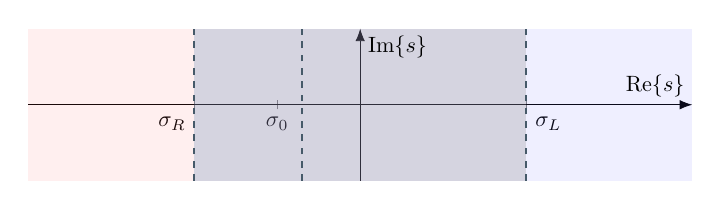
\begin{tikzpicture}[scale=0.8]
                    \begin{axis}[
                        width=\textwidth, height=4cm,
                        axis lines=middle, axis line style={-{Latex[length=2mm]}},
                        xmin=-2, xmax=2, ymin=-2, ymax=2,
                        xtick={-1, -0.5, 1}, xticklabels={$\sigma_R\qquad$, $\sigma_0$, $\qquad\sigma_L$},
                        ytick=\empty,
                        xlabel={$\text{Re}\{s\}$}, ylabel={$\text{Im}\{s\}$}, clip=false
                        ]

                        \fill[blue!60, fill opacity=0.1] (axis cs:-1,-2) rectangle (axis cs:2,2);
                        \fill[red!60, fill opacity=0.1] (axis cs:-2,-2) rectangle (axis cs:1,2);
                        \fill[AccentColor, fill opacity=0.2] (axis cs:-1,-2) rectangle (axis cs:1,2);
                        \draw[dashed, thick, DarkGray] (axis cs:-1,-2) -- (axis cs:-1,2);
                        \draw[dashed, thick, DarkGray] (axis cs:1,-2) -- (axis cs:1,2);
                        \draw[dashed, thick, DarkGray] (axis cs:-0.35,-2) -- (axis cs:-0.35,2);
                    \end{axis}
                \end{tikzpicture}
            \end{center}
            \vspace{-0.2cm}
            \footnotesize
            \begin{itemize}
                \item The ROC of $x(t)$ is the intersection of the ROCs of $x_L(t)$ and $x_R(t)$, which is the region $\sigma_R < \text{Re}\{s\} \le \sigma_L$.
                \item Since $\sigma_0$ is in the ROC, we must have $\sigma_R < \sigma_0 \le \sigma_L$.
                \item Thus, the ROC is a strip in the $s$-plane that includes the line $\text{Re}\{s\} = \sigma_0$.
            \end{itemize}
        \end{column}
    \end{columns}
\end{frame}

\begin{frame}{Example 9.7: A Two-Sided Exponential Signal}
    \begin{columns}[T]
        \begin{column}{0.55\textwidth}
            \begin{itemize}
                \item Signal: $x(t) = e^{-b|t|}$, for $b > 0$.
                \item Since this is a two-sided signal, we can express it as the sum of a right-sided and a left-sided signal:
                      \begin{equation*}
                          x(t) = e^{-bt}u(t) + e^{bt}u(-t)
                      \end{equation*}
                \item From previous examples, the individual transforms are:
                      \begin{align*}
                          e^{-bt}u(t) & \overset{{\mathcal{L}}}{\longleftrightarrow} \frac{1}{s+b}, \quad \text{Re}\{s\} > -b \\
                          e^{bt}u(-t) & \overset{{\mathcal{L}}}{\longleftrightarrow} \frac{-1}{s-b}, \quad \text{Re}\{s\} < b
                      \end{align*}
                \item For the total signal to have a Laplace transform, the two ROCs must overlap. Thus, we require $-b < \text{Re}\{s\} < b$.
                \item If $b \le 0$, there is no common ROC, and the Laplace transform does not exist.
                \item For $b > 0$, combining the transforms gives:
                      \begin{equation*}
                          X(s) = \frac{1}{s+b} - \frac{1}{s-b} = \frac{-2b}{s^2 - b^2}
                      \end{equation*}
                \item \textbf{ROC:} $-b < \text{Re}\{s\} < b$. \quad \textbf{Poles:} $s = \pm b$.
            \end{itemize}
        \end{column}
        \begin{column}{0.45\textwidth}

            \begin{center}
                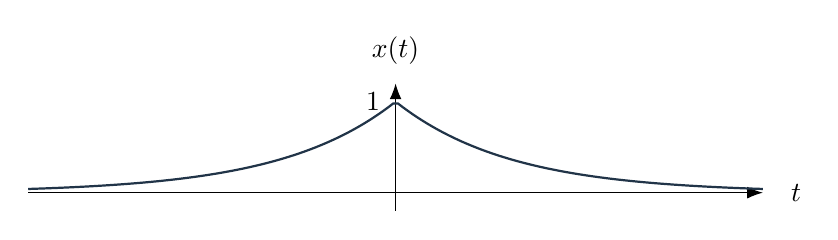
\begin{tikzpicture}
                    \begin{axis}[tick style={draw=none},
                        width=0.9\textwidth, height=3.2cm,
                        axis lines=middle, axis line style={-{Latex[length=2mm]}},
                        xmin=-4, xmax=4, ymin=-0.2, ymax=1.2,
                        xtick=\empty, ytick={1}, yticklabels={$1$},
                        xlabel={$t$}, ylabel={$x(t)$},
                        xlabel style={anchor=west, at={(axis cs:4.2,0)}},
                        ylabel style={anchor=south, at={(axis cs:0,1.3)}},
                        declare function={sig(\t) = exp(-0.8*abs(\t));}
                        ]
                        \addplot[thick, PrimaryColor, domain=-4:4, samples=150] {sig(x)};
                    \end{axis}
                \end{tikzpicture}
            \end{center}

            \begin{center}
                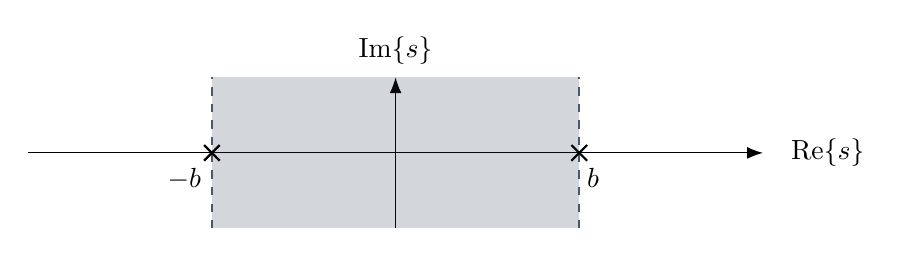
\begin{tikzpicture}
                    \begin{axis}[tick style={draw=none},
                        width=0.9\textwidth, height=3.5cm,
                        axis lines=middle, axis line style={-{Latex[length=2mm]}},
                        xmin=-4, xmax=4, ymin=-2.5, ymax=2.5,
                        xtick={-2, 2}, xticklabels={$-b\qquad$, $\quad b$},
                        ytick=\empty,
                        xlabel={$\text{Re}\{s\}$}, ylabel={$\text{Im}\{s\}$},
                        xlabel style={anchor=west, at={(axis cs:4.2,0)}},
                        ylabel style={anchor=south, at={(axis cs:0,2.6)}},
                        clip=false
                        ]
                        \fill[PrimaryColor, fill opacity=0.2] (axis cs:-2,-2.5) rectangle (axis cs:2,2.5);
                        \draw[dashed, thick, DarkGray] (axis cs:-2,-2.5) -- (axis cs:-2,2.5);
                        \draw[dashed, thick, DarkGray] (axis cs:2,-2.5) -- (axis cs:2,2.5);
                        \addplot[only marks, mark=x, mark options={scale=2, thick}] coordinates {(-2,0) (2,0)};
                    \end{axis}
                \end{tikzpicture}
            \end{center}
        \end{column}
    \end{columns}
\end{frame}

\begin{frame}{ROC Properties 7 and 8: Rational Transforms}
    \begin{tcolorbox}[colframe=PrimaryColor, colback=PrimaryColor!10]
        \textbf{Property 7:} If the Laplace transform $X(s)$ is rational, then its ROC is bounded by poles or extends to infinity. In addition, no poles are contained in the ROC.
    \end{tcolorbox}
    \vspace{0.1cm}
    \textit{Justification:} Rational transforms are combinations of exponentials (we will see this soon).
    And we saw already that the ROC of an exponential is bounded by a pole
    (e.g. $e^{-at}u(t)$ has a pole at $-a$ and the ROC extends from $-a$ to $\infty$).

    As the ROC of a linear combination of signals is the intersection of the ROCs of the individual signals,
    the ROC of a rational transform is bounded by poles or extends to infinity.
    \vspace{0.1cm}

    \begin{tcolorbox}[colframe=PrimaryColor, colback=PrimaryColor!10]
        \textbf{Property 8:} If $X(s)$ is rational, then:
        \begin{itemize}
            \item If $x(t)$ is \textit{right-sided}, the ROC is the region to the \textbf{right of the rightmost pole}.
            \item If $x(t)$ is \textit{left-sided}, the ROC is the region to the \textbf{left of the leftmost pole}.
        \end{itemize}
    \end{tcolorbox}
    \textit{Justification:} Combination of property 4 and 5 with property 7.
\end{frame}

\begin{frame}[fragile]{Example 9.8: One Equation, Three Signals}
    \begin{itemize}
        \item Consider the rational transform: \quad $\displaystyle X(s) = \frac{1}{(s+1)(s+2)}$
        \item Without specifying the ROC, this maps to \textbf{three} possible time-domain signals depending on the bounding poles ($s=-1, -2$):
    \end{itemize}

    \vspace{0.2cm}
    \begin{columns}
        \begin{column}{0.33\textwidth}
            \begin{center}
                \textbf{Right-Sided Signal}\\
                $\text{Re}\{s\} > -1$
                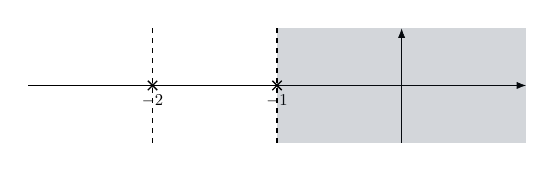
\begin{tikzpicture}[scale=0.6]
                    \begin{axis}[
                        width=\textwidth, height=4cm,
                        axis lines=middle, axis line style={-{Latex[length=2mm]}},
                        xmin=-3, xmax=1, ymin=-2, ymax=2,
                        xtick={-2,-1}, ytick=\empty, clip=false
                        ]
                        \fill[PrimaryColor, fill opacity=0.2] (axis cs:-1,-2) rectangle (axis cs:1,2);
                        \draw[dashed, thick] (axis cs:-1,-2) -- (axis cs:-1,2);
                        \draw[dashed, thick] (axis cs:-2,-2) -- (axis cs:-2,2);
                        \addplot[only marks, mark=x, mark options={scale=2, thick}] coordinates {(-1,0) (-2,0)};
                    \end{axis}
                \end{tikzpicture}
            \end{center}
        \end{column}
        \begin{column}{0.33\textwidth}
            \begin{center}
                \textbf{Left-Sided Signal}\\
                $\text{Re}\{s\} < -2$
                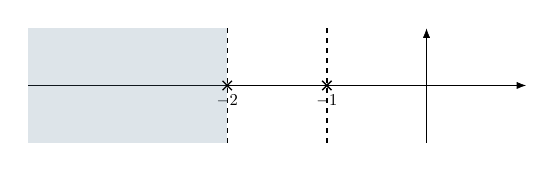
\begin{tikzpicture}[scale=0.6]
                    \begin{axis}[
                        width=\textwidth, height=4cm,
                        axis lines=middle, axis line style={-{Latex[length=2mm]}},
                        xmin=-4, xmax=1, ymin=-2, ymax=2,
                        xtick={-2,-1}, ytick=\empty, clip=false
                        ]
                        \fill[SecondaryColor, fill opacity=0.2] (axis cs:-4,-2) rectangle (axis cs:-2,2);
                        \draw[dashed, thick] (axis cs:-1,-2) -- (axis cs:-1,2);
                        \draw[dashed, thick] (axis cs:-2,-2) -- (axis cs:-2,2);
                        \addplot[only marks, mark=x, mark options={scale=2, thick}] coordinates {(-1,0) (-2,0)};
                    \end{axis}
                \end{tikzpicture}
            \end{center}
        \end{column}
        \begin{column}{0.33\textwidth}
            \begin{center}
                \textbf{Two-Sided Signal}\\
                $-2 < \text{Re}\{s\} < -1$
                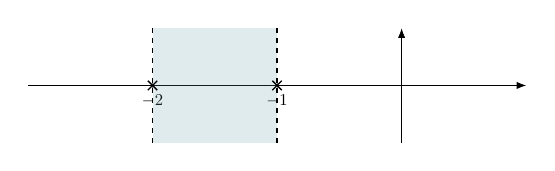
\begin{tikzpicture}[scale=0.6]
                    \begin{axis}[
                        width=\textwidth, height=4cm,
                        axis lines=middle, axis line style={-{Latex[length=2mm]}},
                        xmin=-3, xmax=1, ymin=-2, ymax=2,
                        xtick={-2,-1}, ytick=\empty, clip=false
                        ]
                        \fill[AccentColor, fill opacity=0.2] (axis cs:-2,-2) rectangle (axis cs:-1,2);
                        \draw[dashed, thick] (axis cs:-1,-2) -- (axis cs:-1,2);
                        \draw[dashed, thick] (axis cs:-2,-2) -- (axis cs:-2,2);
                        \addplot[only marks, mark=x, mark options={scale=2, thick}] coordinates {(-1,0) (-2,0)};
                    \end{axis}
                \end{tikzpicture}
            \end{center}
        \end{column}
    \end{columns}
\end{frame}

\section{The Inverse Laplace Transform}

\begin{frame}{The Inverse Laplace Transform: Derivation}
    \begin{itemize}
        \item Recall that we interpreted the Laplace transform of $x(t)$ as the Fourier transform of the exponentially weighted signal $x(t)e^{-\sigma t}$:
              \begin{equation*}
                  X(\sigma + j\omega) = \mathcal{F} \{ x(t)e^{-\sigma t} \} = \int_{-\infty}^{\infty} x(t)e^{-\sigma t} e^{-j\omega t} dt
              \end{equation*}
        \item We can apply the \textbf{Inverse Continuous-Time Fourier Transform} to recover the weighted signal $x(t)e^{-\sigma t}$:
              \begin{equation*}
                  x(t)e^{-\sigma t} = \frac{1}{2\pi} \int_{-\infty}^{\infty} X(\sigma + j\omega) e^{j\omega t} d\omega
              \end{equation*}
        \item Multiplying both sides by $e^{\sigma t}$ yields:
              \begin{equation*}
                  x(t) = \frac{1}{2\pi} \int_{-\infty}^{\infty} X(\sigma + j\omega) e^{(\sigma + j\omega)t} d\omega
              \end{equation*}
    \end{itemize}
\end{frame}

\begin{frame}{The Inverse Laplace Formula}
    \begin{itemize}
        \item Let's perform a change of variables in the integration. We substitute $s = \sigma + j\omega$.
        \item Since $\sigma$ is treated as constant during this integration, the differential becomes $ds = j d\omega$, or $d\omega = \frac{ds}{j}$.
        \item The limits of integration for $\omega$ are $-\infty$ to $+\infty$, which correspond to $s$ running from $\sigma - j\infty$ to $\sigma + j\infty$.
        \item $\sigma$ must be chosen within the ROC of $X(s)$, otherwise $X(s)$ is not defined.
    \end{itemize}

    \vspace{0.3cm}
    \begin{conceptbox}{Inverse Laplace Transform}
        \vspace{-0.2cm}
        \begin{equation*}
            x(t) = \frac{1}{2\pi j} \int_{\sigma - j\infty}^{\sigma + j\infty} X(s) e^{st} ds
        \end{equation*}
        \textit{where  $\sigma$ can be chosen anywhere within the ROC of $X(s)$.}
    \end{conceptbox}
\end{frame}

\begin{frame}{Evaluating the Inverse: Bromwich Integral}
    \begin{columns}[T]
        \begin{column}{0.55\textwidth}
            \begin{itemize}
                \item The equation above is known as the \textbf{Bromwich Integral} or the Mellin inversion formula.
                \item This involves a \textbf{contour integration} in the complex $s$-plane along a straight vertical line $\text{Re}\{s\} = \sigma$.
                \item In practice, this contour is closed along an infinite semicircle to the left or right (depending on $t>0$ or $t<0$), allowing the use of the \textbf{Cauchy Residue Theorem}:
                      \begin{equation*}
                          \oint_C f(s) ds = 2\pi j \sum \text{Residues enclosed by } C
                      \end{equation*}
                \item However, directly evaluating Cauchy residues via contour integrals is mathematically a bit tough.
                \item If you are still interested you can check this video:\\ \url{https://youtu.be/r68zKdyIwVo}
            \end{itemize}
        \end{column}
        \begin{column}{0.45\textwidth}
            \begin{center}
                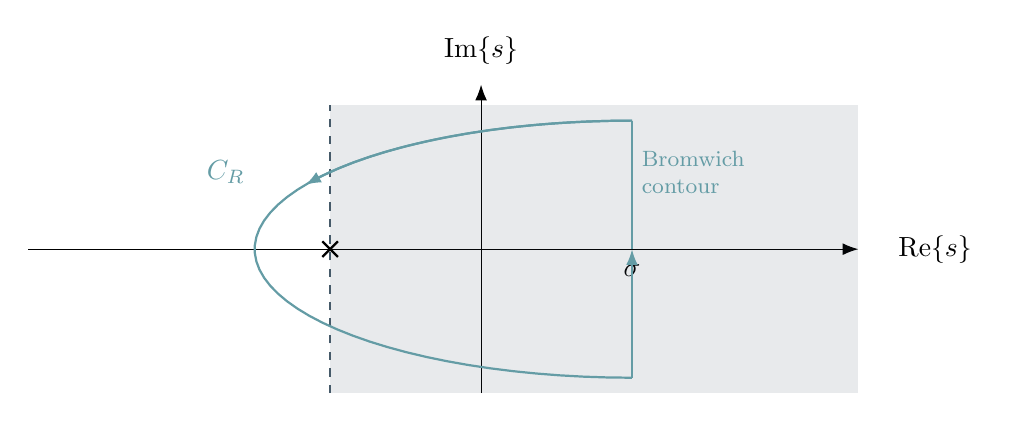
\begin{tikzpicture}
                    \begin{axis}[tick style={draw=none},
                        width=\textwidth, height=5.5cm,
                        axis lines=middle, axis line style={-{Latex[length=2mm]}},
                        xmin=-3, xmax=2.5, ymin=-2.8, ymax=3.2,
                        xtick={1}, xticklabels={$\sigma$},
                        ytick=\empty,
                        xlabel={$\text{Re}\{s\}$}, ylabel={$\text{Im}\{s\}$},
                        xlabel style={anchor=west, at={(axis cs:2.7,0)}},
                        ylabel style={anchor=south, at={(axis cs:0,3.4)}},
                        clip=false
                        ]

                        % ROC
                        \fill[PrimaryColor, fill opacity=0.1] (axis cs:-1,-2.8) rectangle (axis cs:2.5,2.8);
                        \draw[dashed, thick, DarkGray] (axis cs:-1,-2.8) -- (axis cs:-1,2.8);

                        % Pole
                        \addplot[only marks, mark=x, mark options={scale=2, thick}] coordinates {(-1,0)};

                        % Contour
                        % Arc to the left
                        \addplot[thick, AccentColor, domain=90:270, samples=50, variable=\t] ({1 + 2.5*cos(\t)}, {2.5*sin(\t)});
                        \addplot[thick, AccentColor, -{Latex[length=2mm]}, domain=90:150, samples=20, variable=\t] ({1 + 2.5*cos(\t)}, {2.5*sin(\t)});

                        % Straight Line
                        \draw[thick, AccentColor, -{Latex[length=2mm]}] (axis cs:1,-2.5) -- (axis cs:1,0);
                        \draw[thick, AccentColor] (axis cs:1,0) -- (axis cs:1,2.5);

                        % Labels
                        \node[AccentColor, right, align=left] at (axis cs:1, 1.5) {\footnotesize Bromwich\\[-0.5ex] \footnotesize contour};
                        \node[AccentColor, left] at (axis cs:-1.5, 1.5) {$C_R$};
                    \end{axis}
                \end{tikzpicture}
            \end{center}
            \vspace{-0.4cm}
            \begin{center}
                \footnotesize\textit{Contour closed to the left for $t>0$, enclosing poles.}
            \end{center}
        \end{column}
    \end{columns}
\end{frame}

\begin{frame}{Numerical Approximation of Inverse Laplace}
    \begin{itemize}
        \item Sometimes we may not have an analytical inverse, or we only need a numerical approximation of $x(t)$.
        \item Recall that the inverse Laplace transform can be written as an integration over $\omega$:
              \begin{equation*}
                  x(t) = \frac{1}{2\pi} \int_{-\infty}^{\infty} X(\sigma + j\omega) e^{(\sigma + j\omega)t} d\omega
              \end{equation*}
        \item We can approximate this continuous integral with a discrete Riemann sum by taking small frequency steps $\Delta \omega$:
              \begin{equation*}
                  x(t) \approx \frac{1}{2\pi} \sum_{k=-\infty}^{\infty} X(\sigma + jk\Delta \omega) e^{(\sigma + jk\Delta \omega)t} \Delta \omega
              \end{equation*}
    \end{itemize}

    \vspace{0.1cm}
    \begin{insightbox}{Numerical Approx. Inverse Laplace}
        \vspace{-0.2cm}
        \begin{equation*}
            x(t) \approx \frac{\Delta \omega}{2\pi} \sum_{k=-\infty}^{\infty} X(\sigma + jk\Delta \omega) e^{(\sigma + jk\Delta \omega)t}
        \end{equation*}
        $\sigma$ must still be chosen within the ROC.
    \end{insightbox}
\end{frame}

\begin{frame}{Practical Approach: Partial-Fraction Expansion}
    In many real-world problems we are dealing with rational Laplace transforms.
    \begin{itemize}
        \item Instead of using the formal contour integration, we heavily rely on \textbf{Partial-Fraction Expansion}.
        \item For \textit{rational} Laplace transforms $X(s) = \frac{N(s)}{D(s)}$ with simple poles at $s = -a_i$, we expand carefully:
              \begin{equation*}
                  X(s) = \sum_{i=1}^{M} \frac{A_i}{s + a_i}
              \end{equation*}
        \item Because the Laplace transform is linear, we simply invert each first-order term $\frac{A_i}{s+a_i}$ individually.
        \item \textbf{Importantly,} to invert a term, we must know its ROC. There are two distinct time-domain signals for every term $\frac{A_i}{s+a_i}$ depending on the assumed ROC.
    \end{itemize}
\end{frame}

\begin{frame}{The Importance of ROC for Inversion}
    If the fractional term is $\displaystyle \frac{A}{s+a}$:
    \vspace{0.1cm}
    \begin{columns}
        \begin{column}{0.48\textwidth}
            \textbf{ROC is to the right ($\text{Re}\{s\} > -a$)}

            \vspace{0.1cm}
            \begin{center}
                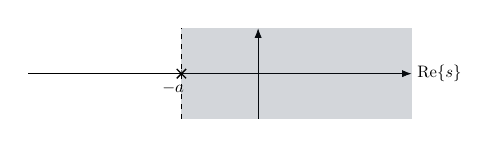
\begin{tikzpicture}[scale=0.6]
                    \begin{axis}[
                        width=0.8\textwidth, height=3.5cm,
                        axis lines=middle, axis line style={-{Latex[length=2mm]}},
                        xmin=-3, xmax=2, ymin=-2, ymax=2,
                        xtick={-1}, xticklabels={$-a\quad$}, ytick=\empty, clip=false,
                        xlabel={$\text{Re}\{s\}$}, xlabel style={anchor=west, at={(axis cs:2,0)}}
                        ]
                        \fill[PrimaryColor, fill opacity=0.2] (axis cs:-1,-2) rectangle (axis cs:2,2);
                        \draw[dashed, thick] (axis cs:-1,-2) -- (axis cs:-1,2);
                        \addplot[only marks, mark=x, mark options={scale=2, thick}] coordinates {(-1,0)};
                    \end{axis}
                \end{tikzpicture}

                \vspace{0.3cm}
                $\frac{A}{s+a} \overset{{\mathcal{L}}}{\longleftrightarrow} A e^{-at}u(t)$

                \vspace{0.3cm}
                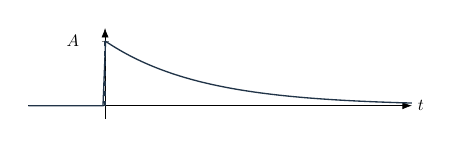
\begin{tikzpicture}[scale=0.6]
                    \begin{axis}[
                        width=0.8\textwidth, height=3.5cm,
                        axis lines=middle, axis line style={-{Latex[length=2mm]}},
                        xmin=-1, xmax=4, ymin=-0.2, ymax=1.2,
                        xtick=\empty, ytick={1}, yticklabels={$A\quad$}, clip=false,
                        xlabel={$t$}, xlabel style={anchor=west, at={(axis cs:4,0)}},
                        declare function={sig(\t) = \t >= 0 ? exp(-0.8*\t) : 0;}
                        ]
                        \addplot[thick, PrimaryColor, domain=-1:4, samples=150] {sig(x)};
                        \draw[dashed, PrimaryColor, thick] (axis cs:0,0) -- (axis cs:0,1);
                    \end{axis}
                \end{tikzpicture}

                \footnotesize\textit{(Right-sided signal)}
            \end{center}
        \end{column}
        \begin{column}{0.48\textwidth}
            \textbf{ROC is to the left ($\text{Re}\{s\} < -a$)}

            \vspace{0.1cm}
            \begin{center}
                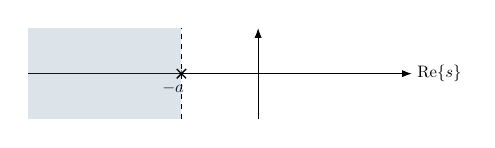
\begin{tikzpicture}[scale=0.6]
                    \begin{axis}[
                        width=0.8\textwidth, height=3.5cm,
                        axis lines=middle, axis line style={-{Latex[length=2mm]}},
                        xmin=-3, xmax=2, ymin=-2, ymax=2,
                        xtick={-1}, xticklabels={$-a\quad$}, ytick=\empty, clip=false,
                        xlabel={$\text{Re}\{s\}$}, xlabel style={anchor=west, at={(axis cs:2,0)}}
                        ]
                        \fill[SecondaryColor, fill opacity=0.2] (axis cs:-3,-2) rectangle (axis cs:-1,2);
                        \draw[dashed, thick] (axis cs:-1,-2) -- (axis cs:-1,2);
                        \addplot[only marks, mark=x, mark options={scale=2, thick}] coordinates {(-1,0)};
                    \end{axis}
                \end{tikzpicture}

                \vspace{0.3cm}
                $\frac{A}{s+a} \overset{{\mathcal{L}}}{\longleftrightarrow} -A e^{-at}u(-t)$

                \vspace{0.3cm}
                \begin{tikzpicture}[scale=0.6]
                    \begin{axis}[
                        width=0.8\textwidth, height=3.5cm,
                        axis lines=middle, axis line style={-{Latex[length=2mm]}},
                        xmin=-4, xmax=1, ymin=-3, ymax=1,
                        xtick=\empty, ytick={-1}, yticklabels={$-A\quad$}, clip=false,
                        xlabel={$t$}, xlabel style={anchor=west, at={(axis cs:1,0)}},
                        declare function={sig(\t) = \t <= 0 ? -exp(-0.6*\t) : 0;}
                        ]
                        \addplot[thick, SecondaryColor, domain=-2:1, samples=150] {sig(x)};
                        \draw[dashed, SecondaryColor, thick] (axis cs:0,0) -- (axis cs:0,-1);
                    \end{axis}
                \end{tikzpicture}

                \footnotesize\textit{(Left-sided signal)}
            \end{center}
        \end{column}
    \end{columns}
\end{frame}

\begin{frame}{Examples 9.9, 9.10, 9.11: Partial Fraction Inversion}
    \begin{itemize}
        \item Let our transform be the system from Example 9.8:
              \begin{equation*}
                  X(s) = \frac{1}{(s+1)(s+2)} = \frac{A}{s+1} + \frac{B}{s+2}
              \end{equation*}
        \item Using the cover-up method or equivalent algebra:
              \begin{align*}
                  A & = \left. (s+1)X(s) \right|_{s=-1} = \left. \frac{1}{s+2} \right|_{s=-1} = 1  \\
                  B & = \left. (s+2)X(s) \right|_{s=-2} = \left. \frac{1}{s+1} \right|_{s=-2} = -1
              \end{align*}
        \item Thus, the expanded form is ALWAYS:
              \begin{equation*}
                  X(s) = \frac{1}{s+1} - \frac{1}{s+2}
              \end{equation*}
    \end{itemize}
\end{frame}

\begin{frame}[fragile]{Example 9.9: Inverting a Right-Sided ROC}
    \begin{itemize}
        \item Suppose the given ROC is \textbf{$\text{Re}\{s\} > -1$}.
        \item By evaluating the overall ROC against each term's pole, we can find the individual ROCs:
              \begin{align*}
                  \text{Pole at } s=-1: & \quad \text{ROC is to the right.} \implies \frac{1}{s+1} \overset{{\mathcal{L}}}{\longleftrightarrow} +e^{-t}u(t)  \\
                  \text{Pole at } s=-2: & \quad \text{ROC is to the right.} \implies \frac{1}{s+2} \overset{{\mathcal{L}}}{\longleftrightarrow} +e^{-2t}u(t)
              \end{align*}
    \end{itemize}
    \vspace{0.2cm}
    \begin{columns}
        \begin{column}{0.5\textwidth}
            \vspace{0.8cm}
            \textbf{Resulting inverse transform:}
            \begin{equation*}
                x(t) = \left(e^{-t} - e^{-2t}\right)u(t)
            \end{equation*}
        \end{column}
        \begin{column}{0.5\textwidth}
            \begin{center}
                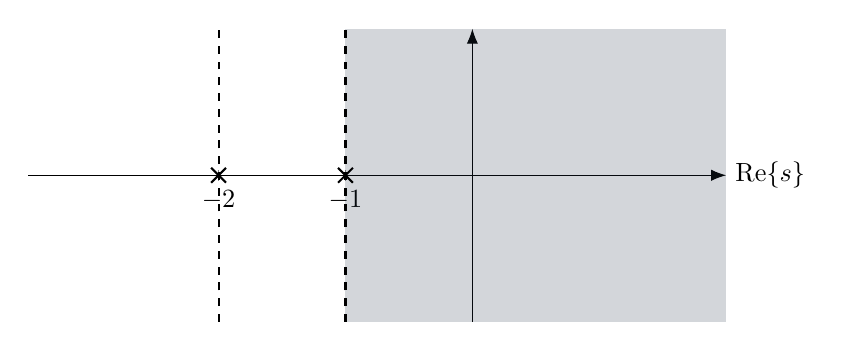
\begin{tikzpicture}[scale=0.95]
                    \begin{axis}[
                        width=0.9\textwidth, height=5.5cm,
                        axis lines=middle, axis line style={-{Latex[length=2mm]}},
                        xmin=-3.5, xmax=2, ymin=-2.5, ymax=2.5,
                        xtick={-2,-1}, ytick=\empty, clip=false,
                        xlabel={$\text{Re}\{s\}$}, xlabel style={anchor=west, at={(axis cs:2,0)}}
                        ]
                        \fill[PrimaryColor, fill opacity=0.2] (axis cs:-1,-2.5) rectangle (axis cs:2,2.5);
                        \draw[dashed, thick] (axis cs:-1,-2.5) -- (axis cs:-1,2.5);
                        \draw[dashed, thick] (axis cs:-2,-2.5) -- (axis cs:-2,2.5);
                        \addplot[only marks, mark=x, mark options={scale=2, thick}] coordinates {(-1,0) (-2,0)};
                    \end{axis}
                \end{tikzpicture}
            \end{center}
        \end{column}
    \end{columns}
\end{frame}

\begin{frame}[fragile]{Example 9.10: Inverting a Left-Sided ROC}
    \begin{itemize}
        \item Now suppose the given ROC is \textbf{$\text{Re}\{s\} < -2$}.
        \item By evaluating the overall ROC against each term's pole, we can find the individual ROCs:
              \begin{align*}
                  \text{Pole at } s=-1: & \quad \text{ROC is to the left.} \implies \frac{1}{s+1} \overset{{\mathcal{L}}}{\longleftrightarrow} -e^{-t}u(-t)  \\
                  \text{Pole at } s=-2: & \quad \text{ROC is to the left.} \implies \frac{1}{s+2} \overset{{\mathcal{L}}}{\longleftrightarrow} -e^{-2t}u(-t)
              \end{align*}
    \end{itemize}
    \vspace{0.2cm}
    \begin{columns}
        \begin{column}{0.5\textwidth}
            \vspace{0.8cm}
            \textbf{Resulting inverse transform:}
            \begin{equation*}
                x(t) = \left(-e^{-t} + e^{-2t}\right)u(-t)
            \end{equation*}
        \end{column}
        \begin{column}{0.5\textwidth}
            \begin{center}
                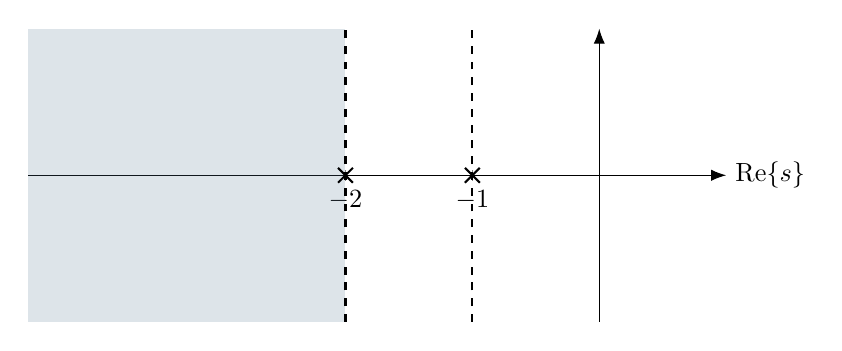
\begin{tikzpicture}[scale=0.95]
                    \begin{axis}[
                        width=0.9\textwidth, height=5.5cm,
                        axis lines=middle, axis line style={-{Latex[length=2mm]}},
                        xmin=-4.5, xmax=1, ymin=-2.5, ymax=2.5,
                        xtick={-2,-1}, ytick=\empty, clip=false,
                        xlabel={$\text{Re}\{s\}$}, xlabel style={anchor=west, at={(axis cs:1,0)}}
                        ]
                        \fill[SecondaryColor, fill opacity=0.2] (axis cs:-4.5,-2.5) rectangle (axis cs:-2,2.5);
                        \draw[dashed, thick] (axis cs:-1,-2.5) -- (axis cs:-1,2.5);
                        \draw[dashed, thick] (axis cs:-2,-2.5) -- (axis cs:-2,2.5);
                        \addplot[only marks, mark=x, mark options={scale=2, thick}] coordinates {(-1,0) (-2,0)};
                    \end{axis}
                \end{tikzpicture}
            \end{center}
        \end{column}
    \end{columns}
\end{frame}

\begin{frame}[fragile]{Example 9.11: Inverting a Two-Sided ROC}
    \begin{itemize}
        \item Finally, suppose the ROC is \textbf{$-2 < \text{Re}\{s\} < -1$}.
        \item By evaluating the overall ROC against each term's pole, we can find the individual ROCs:
              \begin{align*}
                  \text{Pole at } s=-1: & \quad \text{ROC is to the left.} \implies \frac{1}{s+1} \overset{{\mathcal{L}}}{\longleftrightarrow} -e^{-t}u(-t)  \\
                  \text{Pole at } s=-2: & \quad \text{ROC is to the right.} \implies \frac{1}{s+2} \overset{{\mathcal{L}}}{\longleftrightarrow} +e^{-2t}u(t)
              \end{align*}
    \end{itemize}
    \vspace{0.2cm}
    \begin{columns}
        \begin{column}{0.5\textwidth}
            \vspace{0.8cm}
            \textbf{Resulting inverse transform:}
            \begin{equation*}
                x(t) = -e^{-t}u(-t) - e^{-2t}u(t)
            \end{equation*}
        \end{column}
        \begin{column}{0.5\textwidth}
            \begin{center}
                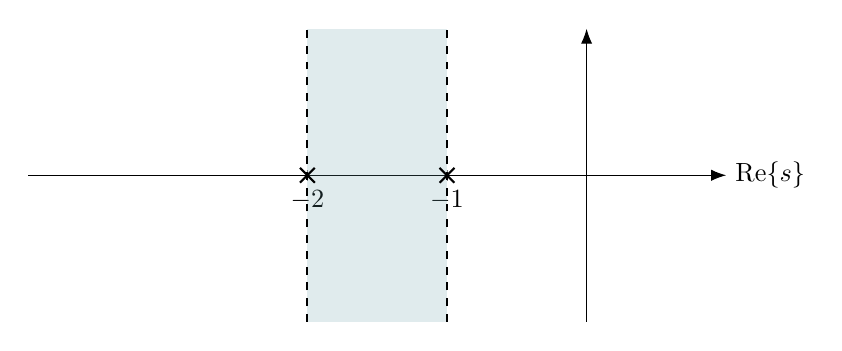
\begin{tikzpicture}[scale=0.95]
                    \begin{axis}[
                        width=0.9\textwidth, height=5.5cm,
                        axis lines=middle, axis line style={-{Latex[length=2mm]}},
                        xmin=-4, xmax=1, ymin=-2.5, ymax=2.5,
                        xtick={-2,-1}, ytick=\empty, clip=false,
                        xlabel={$\text{Re}\{s\}$}, xlabel style={anchor=west, at={(axis cs:1,0)}}
                        ]
                        \fill[AccentColor, fill opacity=0.2] (axis cs:-2,-2.5) rectangle (axis cs:-1,2.5);
                        \draw[dashed, thick] (axis cs:-1,-2.5) -- (axis cs:-1,2.5);
                        \draw[dashed, thick] (axis cs:-2,-2.5) -- (axis cs:-2,2.5);
                        \addplot[only marks, mark=x, mark options={scale=2, thick}] coordinates {(-1,0) (-2,0)};
                    \end{axis}
                \end{tikzpicture}
            \end{center}
        \end{column}
    \end{columns}
\end{frame}

\end{document}
